\documentclass[11pt]{upenndiss}

%bibliography
\usepackage{natbib}
\bibpunct[:]{(}{)}{,}{a}{}{,}

\usepackage[all]{xypic}
% phonological examples


% fonts
\usepackage{fontspec}
%\usepackage{mathspec}
%\setmainfont[Mapping=tex-text]{Linux Libertine}
%\setmathfont(Digits,Greek,Latin){Linux Libertine}
%\usepackage{microtype}
%\usepackage{coptic}

\usepackage{setspace}

% tables and figures
\usepackage{booktabs}
\usepackage{floatrow}
\usepackage{enumitem}
\setlist{noitemsep}
\usepackage{multirow,sectsty}
\usepackage{subfigure,graphicx}

% Add packages and definitions you want to use here:
\usepackage[papersize={8.5 in, 11 in}, nohead, includeheadfoot, left=1.5 in, right = 1 in, vmargin= 1 in]{geometry}

%\usepackage{times}


%\usepackage{tipa}




% titles
\title{Parameterising Germanic ditransitive variation:\newline A historical-comparative study}
\author{Hezekiah Akiva Bacovcin}
\supervisor{Anthony Kroch}

\copyrighttrue
\department{Linguistics}

% Abstract
\abstractfile{Abstract} 
% Acknowledgement
\acknowledgementsfile{Acknowledgements}

% Dedication
%\dedication{
%}



\usepackage{gb4e}
\noautomath

\begin{document}

\thispagestyle{empty}\enlargethispage{\the\footskip}%
\null\vskip.1in%
\begin{center}
        {\setstretch{2.5} \MakeUppercase{Parameterising Germanic ditransitive variation}\par }%
        \vskip.3in
        Hezekiah Akiva Bacovcin
        \vskip .3in
        A DISSERTATION \\[.1in]
        in \\[.1in]
        Linguistics
        \vfill
Presented to the Faculties of the University of Pennsylvania in Partial \\
Fulfillment of the Requirements for the Degree of Doctor of Philosophy
\\[0.3in]
        2016
  \end{center}
  
  \parbox[t]{12cm}{\parindent=0pt Supervisor of Dissertation \vskip 0.5in
  \par \hrule width 7cm \vskip .1in Anthony Kroch, Professor of  Linguistics}
  
  \vskip 0.3in
  
  \parbox[t]{12cm}{\parindent=0pt Graduate Group Chairperson \vskip 0.5in
  \par \hrule width 7cm \vskip .1in Rolf Noyer, Associate Professor of Linguistics}

  \vskip 0.3in
  
  \parbox[t]{12cm}{\parindent=0pt Dissertation committee 
  \vskip -.1in
  David Embick, Professor of Linguistics
  \vskip -.1in
  William Haddican, Associate Professor of Linguistics, CUNY
  \vskip -.1in  
  Julie Legate, Professor of Linguistics
  \vskip -.1in
  Don Ringe, Professor of Linguistics
  }



\newpage 


\FrontMatter

% {\addcontentsline{toc}{chapter}{\listtablename}\listoftables}

%%%%%%%%%
\part{Introduction}
\chapter{Introduction}
\label{ch:introduction}

This dissertation argues for two main conclusions. First, we provide evidence suggesting that all Germanic languages have the same base generation structure for recipient ditransitives (namely recipient--theme) with theme--recipient orders derived by scrambling. Part of this argument entails that prepositional object constructions (e.g. "John gave the book to Mary") in languages like English should be analysed in the same way as scrambled accusative--dative structures in languages with overt case marking. This conclusion supports syntactic unification of prepositions and (inherent) case markers (INSERT CITATIONS HERE). Secondly, we argue that symmetric passivization with ditransitives (INSERT CITATIONS HERE) are derived by parameterising the relationship between nominative case assignment and movement to subject position. This parameter interacts with the availability of dative--to--nominative conversion to create the surface patterns of passivisation found in the Germanic languages.

The dissertation relies on comparative and historical evidence from Germanic languages. English is one of the languages for which the largest number of resources exist for studying historical syntax (i.e. the largest number of parsed corpora). By studying other Germanic languages that are closely related to English, it is possible to see whether small changes in the syntactic make-up of a language impacts the languages ditransitive syntax. An overview of the different Germanic languages can be found in CITATION. The following syntactic variants are found in the Germanic languages: the absence/presence of V2 (English/all other languages), VO vs OV (Modern English and Scandinavian vs Old English, German, Dutch and Afrikaans), and the absence/presence of synthetic dative case (Modern English, standard mainland Scandinavian, Dutch, Afrikaans, Low German vs Old English, German, Yiddish, Icelandic, Faroese and some Scandinavian dialects). During the dissertation, I will show how they analysis of ditransitives correlates (or does not correlate) with these differences. 

The outline of the dissertation is as follows. In this chapter, I start by introducing the topic of the dissertation and presents an outline of its structure. In the following section (Sec. REFERENCE), I motivate focusing the dissertation on recipient ditransitives in Germanic langauges. I show that recipient ditransitives are a separate class of ditransitives from benefactive, goal and addressee ditransitives and argue that recipient ditransitives form the core ditransitive category and demonstrate why they are the focus of the rest of the dissertation.

In the next chapter, I argue that all Germanic languages share the same base generated structure for recipient ditransitives (namely dative--accusative). Following CITATION, who argues that inherent dative case and prepositions represent the same syntactic category, I present an analysis of English that unifies dative shift (i.e. the derivation of ``I gave the book to John'') with VP-internal scrambling proposed for the derivation of accusative--dative orders in German (CITATION). This leads to the conclusion that in non-scrambled environments the recipient should always asymmetrically c-command the theme.

In chapter 3, I discuss the role of locality in ditransitive passives. I present evidence that the case assignment/agreement and movement properties of subjecthood can show different locality properties. I will also discuss how these properties intersect with the possibility of dative--to--nominative raising in passives.

Finally, in chapter 4, I present a formal implementation of the analysis from chapter 2 and 3 in the minimalist/distributed morphology framework, discuss relevant cases of historical change and their implication for broader theories of historical change, and conclude with a discussion of further implications (especially with respect to ergativity).

\part{Active Ditransitives}
\chapter{Base generation and srambling}\label{ch:base-gen}
This part of the dissertation focuses on identifying and analysing the core case of ditransitives. The first chapter argues that there are (at least) three distinct ditransitive constructions (as seen on the surface in languages like German): dative--accusative ditransitives, accusative--dative ditransitives, and prepositional object constructions. Following others in the literature, I argue that accusative--dative ditransitives are derived from dative--accusative ditransitives via scrambling (i.e. only dative--accusative ditransitives and prepositional object constructions are base generated). In this chapter, I also describe why the dissertation focuses on recipient ditransitives (instead of, for example, benefactives). The next few chapters introduce the idea that the output of dative shift operations in languages that have them (e.g. `John gave the book to Mary') should be analysed as cases of accusative--dative ditransitives and not prepositional object constructions (in spite of their surface similarity to prepositional object constructions). 
\section{Introduction to Germanic Recipient Ditransitives}
All of the Germanic languages can introduce recipients in ditransitive clauses without the use of prepositions. In languages with synthetic case marking (Icelandic, Faroese, some Norwegian dialects, Yiddish and High German), the recipient is marked with dative case.

\begin{exe}
\ex
\begin{xlist}
\ex Icelandic:
\gll P\'{e}tur gaf konunginum amb\'{a}ttina.\\
Peter.NOM gave king.DEF.DAT maid-servant.DEF.ACC.\\
\trans `Peter gave the king the maid-servant.'
\ex Faroese:
\gll Hon gav Mariu troyggiuna.\\
She gave Maria.DAT sweater.DEF.ACC.\\
\trans `She gave Maria the sweater \citep{Lundquist.2013b}.'
\ex Standard Norwegian:
\gll Jeg har gitt mannen boken.\\
I have given man.DEF book.DEF.\\
\trans `I gave the man the book \citep[ex 10]{Sprouse.1995}.'
\ex Halsa Norwegian (dialect):
\gll Ho ga kattåinn mat.\\
she gave cat.DEF.DAT food.\\
\trans `She gave the cat food \citep{Afarli.2012}.'
\ex Swedish:
\gll Jag gav Johan en bok.\\
I gave John a book.\\
\trans `I gave John a book \citep{Holmberg.1995}.'
\ex Danish:
\gll Peter viste jo Marie bogen.\\
Peter showed indeed Mary book.DEF.\\
\trans `Peter indeed showed Mary the book \citep{Vikner.1989}.'
\ex High German:
\gll weil er (der) Unehrlichkeit keine Chance gibt.\\
as he.NOM (the) dishonesty.DAT no opportunity.ACC gives.\\
\trans `as he gives dishonesty no opportunity \citep[162]{Draye.1996}.'
\ex Yiddish:
\gll Zi git der snjjer dus pékl. \\
she.NOM gives the.DAT daughter-in-law the.ACC parcel.\\
\trans 'She gives her daughter-in-law the parcel \citep[ex 190a]{Birnbaum.1979}.'
\ex Dutch:
\gll Ik heb (aan) Jan een boek gegeven.\\
I have (to) Jan a book given.\\
\trans `I gave Jan a book \citep{Tiersma.1985}.'
\ex Afrikaans:
\gll dat die man die vrou `n dokument gegee het.\\
that the man the woman a document given has.\\
\trans `...that the man gave a document to the woman \citep{Louw.2012}.'
\ex Frisian:
\gll se joech jar kammeraatske in skjirre.\\
she gave her girlfriend a {pair of scissors}.\\
\trans `She gave her girlfriend a pair of scissors.'
\ex Low German: 
\gll ick gaw den Mann dat Brod.\\
I gave the man the bread.\\
\trans `I gave the man the bread \citep{Mussaus.1829}.'
\ex English: I gave the man the book.
\end{xlist}
\end{exe}

Most of the Germanic languages also allow recipients to be introduced with a preposition and require the preposition in theme--recipient orders. One of the main points of the next few chapters is to determine the relationship between prepositional and non-prepositional recipients.

\begin{exe}
	\ex \label{ex:preprec}
	\begin{xlist}
		\ex Norwegian:
		\gll Vi har lånt den interessante boken du nevnte *(til) Petter.\\
		we have lent the interesting book you mentioned to Peter.\\
		\trans `We have lent the interesting book you mentioned to Peter \citep{Larson.1988}.'
		\ex Swedish:
		\ex \gll Jag gav en bok *(til) Johan.\\
		I gave a book to John.\\
		\trans `I gave a book to John \citep{Holmberg.1995}.'
		\ex Danish:	
		\gll Jeg gav bogen *(til) Anna.\\
		I gave book.the to Anna.\\
		\trans `I gave the book to Anna\citep{Holmberg.1998}.'
		\ex Dutch:
		\gll Ik heb een boek *(aan) Jan gegeven.\\
		I have a book *(to) Jan given.\\
		\trans `I gave a book to Jan.'
		\ex Afrikaans: 
		\gll Ek het `n fooitjie aan hom gegee.\\
		I have a tip to him given.\\
		\trans `I have given a tip to him \citep{Stadler.1996}.'
		\ex Frisian:
		\gll ik joech in plant oan Beppe.\\
		I gave a plant to Grandmother.\\
		\trans `I gave a plant to Grandmother \citep{Tiersma.1985}.'
		\ex English: I gave the book to the man.
	\end{xlist}
\end{exe}

Most of the languages with synthetic case marking for which I have data do not allow recipients to be introduced by a preposition. For Icelandic\footnote{Icelandic does allow `til' with verbs like GIVE, but only with inanimate objects with an idiomatic donation reading. \cite{Thrainsson.2007} claims that this can only occur when `a goal interpretation can be coerced.'
\begin{exe}
	\ex \gll J\'on gaf b\'okasafn sitt til h\'ask\'olans.\\
	John gave library {his own} to university.DEF.\\
\trans `John donated his own library to the university.'
\end{exe}} and German, the following examples show how prepositional recipients are ungrammatical. For Yiddish, I do not have ungrammatical examples, but there is no discussion of the possibility of prepositional recipients in the grammars (e.g. \citet{Birnbaum.1979}).

\begin{exe}
	\ex
	\begin{xlist}
		\ex Icelandic:
	\gll *J\'on gaf b\'okina til Mar\'iu.\\
		 John gave book.DEF to Mary.\\
		 \trans `John gave the book to Mary.'
		\ex Standard High German:
		\gll *Jan hat das Buch an Maria gegeben.\\
		 John has the book to Maria given.\\
		 \trans `John gave the book to Mary.'
	\end{xlist}
\end{exe}

While the availability of prepositional recipients tends to correlate with the absence of synthetic dative case, there are examples of languages with synthetic dative case that have prepositional case marking (Faroese and High German Dialects) and there is an example of a language without synthetic case that does not have prepositional recipients (Low German). 

Both of the languages with synthetic dative case that allow prepositional recipients have been in intense contact with languages that have prepositional recipients. Faroese has been in intense contact Danish for the last 400 years, while the relevant High German dialects have been in contact with various Romance varieties (French and Northern Italian). This acceptance of prepositional recipients is a recent change in Faroese \citep{Thrainsson.2007,Lundquist.2013b}.

\begin{exe}
	\ex Faroese:
	\gll *?Hon gav telduna til gentuna.\\
	she gave computer-the.ACC to girl-the.ACC.\\
	\trans `She gave the computer to the girl.'
	\ex Bavarian German:
	\gll gib-s a da Kathi.\\
	give-it to the.DAT Kathy.\\
	\trans `Give it to Kathy \citep[pg 95]{Seiler.2003}!'
\end{exe}

Concerning Low German, \cite{Fleischer.2006} states: ``In Low German, this construction [prepositional dative marking] could eventually be viewed as compensatory to the loss of a distinct dative case; however, from the fact that I could not find any decisive examples of this construction in Low German, I conclude that it is very rare.'' \cite{Lindow.1998} makes no mention of prepositional dative marking (including in a section discussing the uses of various prepositions. However, \cite{Mussaus.1829} gives examples of theme--recipient clauses without any prepositional marking, even though the dative/accusative distinction had been lost hundreds of years before Mussäus wrote his grammar \citep{Lasch.1914,Boden.1993}.

\begin{exe}
	\ex Low German:
	\gll ick gaw dat Brod den Man, wobei dat Brod zeigend ist.\\
	I gave the bread the man who the bread shown is.\\
	\trans `I gave the bread to the man who was shown the bread \citep{Mussaus.1829}.'
\end{exe}

The remainder of this chapter argues that recipient ditransitives are base generated in a recipient--theme order, with the theme--recipient order derived via scrambling, why recipient ditransitives form a distinct category from other ditransitives, and why recipient ditransitives are the focus of this dissertation (namely that recipient ditransitives are the core ditransitive category with other ditransitives being marginal).
\section{Evidence for Scrambling}

As mentioned above, all of the languages allow bare or dative marked recipients to preceed bare or accusative marked themes. Most of the languages also allow for theme--recipient orders (either with the same case marking pattern or with prepositional marking of the recipient). The prepositionally marked examples were shown above (\ref{ex:preprec}). I show here the theme--recipient order in High German.

\begin{exe}
		\ex High German:
		\gll dann hat die Frau das Buch dem Jungen gegeben\\
		then has the woman.NOM the book.ACC the boy.DAT given\\
		`then the woman has given the book to the boy \citep[ex 1b]{Czepluch.1990}, \citep[20b]{Choi.1996}'
\end{exe}

However, Modern Icelandic does not allow theme--recipient orders (except as the product of heavy NP shift \citep{Dehe.2004}.

\begin{exe}
\ex Icelandic:
\gll ?*Hann gaf amb\'attina konunginum.\\
He.NOM gave maid-servant.DEF.ACC king.DEF.DAT. \\
\trans `He gave the king the maid-servant \citep[ex 14b]{Dehe.2004}.'
\end{exe}

The universality of the recipient--theme order and the unavailability of theme--recipient orders in some languages suggest that the recipient--theme order is basic and the theme--recipient order derived (with Modern Icelandic lacking the theme--recipient deriving transformation). \cite{Georgala.2011} provides evidence from stranded depictives, floating quantifiers and split topics that support the notion that the recipient--theme order is basic. Modern German provides additional evidence that the transformation under discussion is scrambling \citep{Lenerz.1977,Abraham.1986,Webelhuth.1992,Choi.1996}.

\cite{Lenerz.1977} showed that all scrambling in German is sensitive to information focus (i.e. the focus recieved by new information), but contrastive focus can be placed on any element. In particular, words that recieve new information focus cannot be targeted by scrambling operations. \cite{Lenerz.1977} applied this heuristic to ditrasntives and discovered that recipient ditransitives had the following pattern. When recipients recieved information focus (by being the answer to a wh-question), both recipient--theme and theme--recipient word orders were possible. This would be consistent with either of the following analyses: the two word orders are not derived via scrambling or the recipient is not the element that scrambles.

\begin{exe}
\ex IO Focus \citep{Choi.1996}:
\begin{xlist}
\ex \gll Wem hast du das Geld gegeben?\\
whom.DAT have you.NOM the money.ACC given\\
\trans `Who did you give the money to?'
\begin{xlist}
\ex \gll Ich habe dem KASSIERER das Geld gegeben.\\
I.NOM have the cashier.DAT the money.ACC given.\\
\trans `I have given the cashier the money.'
\ex \gll Ich habe das Geld dem KASSIERER gegeben.\\
I.NOM have the money.ACC the cashier.DAT given.\\
\trans `I have given the money to the cashier.'
\end{xlist}
\end{xlist}
\end{exe}

However, when the theme recieves information focus, only the recipient--theme word order is possible. Given the constraints on scrambling in German, this indicates that the recipient--theme order is base generated and that the theme--recipient order is derived via scrambling the theme above the recipient.

\begin{exe}
	\ex DO Focus \citep{Choi.1996}:
\begin{xlist}
\ex \gll Was hast du dem Kassierer gegeben?\\
what.ACC have you.NOM the cashier.DAT given\\
\trans `What did you give to the cashier?'
\begin{xlist}
\ex \gll Ich habe dem Kassierer das GELD gegeben.\\
I.NOM have the cashier.DAT the money.ACC given.\\
\trans `I have given the cashier the money.'
\ex[?*] {Ich habe das GELD dem Kassierer gegeben.}
I.NOM have the money.ACC the cashier.DAT given.\\
\trans `I have given the money to the cashier.'
\end{xlist}
\end{xlist}
\end{exe}

Another piece of evidence about scrambling has to do with the availability of reconstruction. German shows a bias towards surface scope, such that a quantifier needs to c-command any bound pronouns on the surface. This can be seen in the recipient--theme order, where there is no availability of reconstruction (since no movement has taken place).

\begin{exe}
	\ex 
\begin{xlist}
\ex[ ]{\gll dass Maria jedem seinen Nachbarn vorgestellt hat.\\
that Maria everyone.DAT his.ACC neighbour.ACC introduced has.\\
\trans `that Maria introduced everyone his neighbor \citep[ex. 11a]{Lee.1994}.'}
\ex[*]{\gll dass Maria seinem Nachbarn jeden vorgestellt hat.\\
	that Maria his.DAT neighbour.DAT everyone.ACC introduced had.\\
	\trans `that Maria introduced everyone to his neighbour \citep[ex. 9a]{Lee.1994}.'}
\end{xlist}
\end{exe}

In the theme--recipient order, the theme can easily scope over/bind into the recipient. However, the recipient is also able to marginally scope over/bind into the theme. The judgements here are subject to speaker variation, but there are some speakers who allow the scrambled theme to reconstruct (for example to prevent a weak crossover violation). This is consistent with the idea that the theme has moved from a position under the recipient and can (marginally) reconstruct to that position at LF.

\begin{exe}
	\ex High German, theme--recipient 
\begin{xlist}
	\ex[ ]{\gll dass Maria jeden seinem Nachbarn vorgestellt hat.\\
	that Maria everyone.ACC his.DAT neighbour.DAT introduced had.\\
	\trans `that Maria introduced everyone to his neighbour \citep[ex. 10a]{Lee.1994}.'}
	\ex[\%]{\gll dass Maria seinen Nachbarn jedem vorgestellt hat.\\
	that Maria his.ACC neighbour.ACC everyone.DAT introduced had.\\
	\trans `that Maria introduced everyone his neighbour \citep[ex. 12a (note 10)]{Lee.1994}.'}
\end{xlist}
\end{exe}

Two different diagnostics show that the landing site of the scrambling is within the verb phrase. First, in cases of VP-topicalisation, both word orders are possible.

\begin{exe}
	\ex High German, VP-topicalisation:
	\begin{xlist}
		\ex \gll  Dem Mann das Buch gegeben habe ich, (nicht der Frau dEN Film geschenkt).\\
		the.DAT man the.ACC book given have I, (not the.DAT woman the.ACC film sent).\\
		\trans `It was giving the man the book that I did (not sending the woman the film).'
		\ex \gll Das Buch dem Mann gegeben habe ich, (nicht dEN Film der Frau geschenkt).\\
		the.ACC book the.DAT man given have I, (not the.ACC film the.DAT woman sent).\\
		\trans `It was giving the book to the man that I did (not sending the film to the woman).\\
	\end{xlist}
\end{exe}

Secondly, both word orders can occur after VP-level adverbs (such as negation).

\begin{exe}
	\ex High German, VP-level adverbs:
	\begin{xlist}
		\ex \gll Ich habe nicht dem Mann das Buch gegeben, SONDERN DER FRAU DEN FILM GESCHENKT.\\
		I have not the.DAT man the.ACC book given, but the.DAT woman the.ACC film sent.\\
		\trans `I didn't give the man the book, instead I sent the woman the film.'
		\ex \gll Ich habe nicht das Buch dem Mann gegeben, SONDERN DEN FILM DER FRAU GESCHENKT.\\
		I have not the.ACC book the.DAT man given, but the.ACC film the.DAT woman sent.\\
		\trans `I didn't give the book to the man, insead I sent the film to the woman.'
	\end{xlist}
\end{exe}

This section argued that the recipient--theme order is base generated. High German provided evidence that the theme--recipient order was derived via scrambling. In the following section, I will show that these two constructions (base generated recipient--theme and scrambled theme--recipient) are distinct from prepositional object constructions. I also argue for why recipient ditransitives are the focus of this dissertation.

\section{Discursus on Non-Recipient Ditransitives}

The purpose of this section is to explain why this dissertation focuses on recipient ditransitives. There are two main reasons to prefer recipients for the purpose of this investigation in comparison to alternative structures. First, since this dissertation focuses on a comparison across a wide variety of languages, it is essential that the constructions under investigation not be marginal, so that they can be assured to exist in as many of the languages as possible for comparison. I show that many of the alternative ditransitive structures are actually quite marginal and therefore only occur in a sample of the languages. 

One of the other purposes of this dissertation is to investigate the relationship between prepositional object constructions, non-prepositional ditransitive constructions and the results of dative shift operations (for the languages that have them). In the next part of the dissertation, I argue that dative shifted examples need to be taken in to account when discussing the typology of ditransitive passivisation. I show that many of the non-recipient constructions show alternations with prepositional object constructions even in languages with synthetic case marking. Fiven that there are independent sources for prepositional objects in these cases, the rise of dative shift operations there is an ambiguity between the pre-dative shift prepositional objects and the results of dative shift. This ambiguity is avoided by focusing on constructions involving recipients introduced by verbs of transfer (e.g. GIVE) and verbs of future transfer (e.g. PROMISE). One of the themes of this dissertation is to argue that by attempting to collapse a number of distinct constructions together (whose distinctions are seen on the surface in many of the languages with synthetic case marking), deeper generalisations about the individual constructions have been missed (especially with regards to the typology of ditrasitive passivisation).

I start this section by providing a discussion of alternative ditransitive structures in some of the languages with synthetic case marking (Icelandic and Old English). I show that these alternative patterns are: always marginal in comparison to dative--accusative structures, often co-occur with over prepositional object constructions, and tend to behave more like prepositional object constructions even when the prepositions are absent (e.g. resistance to reordering of objects and a theme--indirect object order). I then discuss benefactives and show how they also show covariation with a prepositional construction in all languages, tend to be quite marginal and that non-prepositional forms are ungrammtical/extremely restricted in many of the Germanic languages, which hinders comparison. Finally, I show that verbs of motion and verbs of speaking are also somewhat variable in their ability to license recipients and that even when they do license recipients there is often ambiguity between goal/addressee and recipient interpretations that complicates the investigation of the relationship between prepositional and non-prepositional recipients and the relationship between synthetic dative case and prepositional recipient marking.

\subsection{Prepositional Objects and Alternative Case Patterns}
As seen above, languages with synthetic case marking have dative case marked recipients and accusative case marked themes. In addition to these case marked ditransitives, all languages attest prepositional object ditransitives. In these cases, a (usually accusative) theme is followed by a prepositional phrase. Unlike with recipient constructions, however, variation in word order between the theme and the prepositional object is more marked.

In German, for example, only the theme--prepositional object order is available in VP-topicalisation contexts.

\begin{exe}
	\ex High German, VP-topicalisation:
	\begin{xlist}
		\ex[*]{\gll Nach Paris das Buch geschenkt habe ich, (nicht nach London dEN Film verschifft).\\
		To Paris the.ACC book sent have I, (not to London the.ACC film shipped).\\
		\trans `It was sending to Paris the book that I did (not shipping to London the film).'}
		\ex[ ]{\gll Das Buch nach Paris geschenkt habe ich, (nicht dEN Film nach London verschifft).\\
		the.ACC book to Paris sent have I, (not the.ACC film to London shipped).\\
		\trans `It was sending the book to Paris that I did (not shipping the film to London).'}
	\end{xlist}
\end{exe}

In addition to prepositional objects and dative--accusative recipient ditransitives, many of the languages with synthetic case marking have other ditransitive types that involve different case marking patterns. For example, Icelandic has the following case marking patterns \citep[4.149]{Thrainsson.2007}: dative--accusative, accusative--dative, dative--genitive, dative--dative, and accusative--genitive. Even in older varieties of Icelandic, where theme--recipient word orders were possible with dative--accusative verbs, the other case patterns did not allow for alternate word orders \citep{Ottosson.1991}. Also, many of these other case patterns have prepositional object alternates, which as discussed above do not exist for dative--accusative verbs \citep{Ottosson.1991,Thrainsson.2007}.

Old English attests at least four additional case patterns in addition to the dative recipient/accusative theme pattern discussed above. Note that the same verb can sometimes introduce two different case patterns. \cite{Allen.1999} could not find enough examples of these alternative case patterns in her corpus to identify word order patterns, which suggests that these patterns are marginal compared to the more robust dative recipient/accusative theme pattern.

\begin{table}[h!]
	\begin{tabular}{lll}
		\hline
		THEME & RECIPIENT & Example\\
		\hline
		Accusative & Dative & \emph{giefan} `give'\\
		Genitive & Dative & \emph{forwyrnan} `forbid'\\
		Genitive & Accusative & \emph{bereafian} `deprive'\\
		Accusative & Accusative & \emph{laeran} `teach'\\
		Dative & Accusative & \emph{bereafian} `deprive'\\
		\hline
	\end{tabular}
	\caption{Case-marking patterns of ditransitive verbs in Old English \citep[Table 2.1]{Allen.1999}}
\end{table}

Most of these alternative patterns seem to be marginal. Even in languages that maintain the morphological expression of case, many of these constructions are replaced with prepositional objects. For example, in Modern Faroese, many of the patterns with non-dative recipients or non-accusative themes are being replaced with prepositional objects \citep{Hoskuldurrainsson.2004}. The verb ASK in Old Norse had an accusative phrase followed by a genitive phrase, but in Modern Faroese, it now introduces either two accusative phrases or an accusative phrase and a prepositional object.

\subsection{Benefactive Ditransitives}

In addition to pure recipient interpretations, English double objects also permit benefactive interpretations. These can be identified by the fact that they alternate with a phrase introduced by `for' instead of `to'.

\begin{exe}
	\ex Recipients:
	\begin{xlist}
		\ex[ ]{John gave Mary the book.}
		\ex[ ]{John gave the book to Mary.}
		\ex[*]{John gave the book for Mary.}
	\end{xlist}
	\ex Benefactives:
	\begin{xlist}
		\ex[ ]{John baked Mary the cake.}
		\ex[*]{John baked the cake to Mary.}
		\ex[ ]{John baked the cake for Mary.}
	\end{xlist}
\end{exe}

Phrases introduced by `for' have a much broader scope than bare benefactives. In English, bare benefactive require a (potential) recipient relationship (i.e. the theme needs to be at least intended for the beneficiary).

\begin{exe}
	\ex John baked Mary a cake.
	\begin{xlist}
		\ex[ ]{John baked a cake so that Mary would have one.}
		\ex[*]{John baked a cake so that Mary would fulfill her cake making obligation.}
	\end{xlist}
\end{exe}

Thus, the benefactives in English require a theme in order to be licensed (since there must be an object whose possession is under discussion). This contrasts with other languages with true benefactives (i.e. any type of beneficiary). 

\begin{exe}
	\ex Albanian:
	\gll Agimi i mban Drit\"es {\c{c} anten} time.\\
	Agim.NOM CL holds Drita.DAT bag.ACC my\\
	\trans `Agim holds my bag for Drita \citep[ex 8a]{McGinnis.2001b}.'
\end{exe}

Phrases marked with `for' pattern like true benefactives in co-occuring with intransitive predicates.

\begin{exe}
	\ex John ran *(for) the charity.
\end{exe}

All of the Germanic languages have a cognate of `for' that behaves like a true benefactive and as a prepositional object (i.e. with the standard order being object--prepositional phrase). This contrasts with recipients, as discussed above, in so far as most languages with synthetic dative case do not allow recipients to be introduced in prepositional phrases.
%\begin{exe}
%	\ex 
%	\begin{xlist}
%		\ex Icelandic:
%		\gll  
%		\ex Dutch:
%		\gll Jan bakte een taart voor Mary.\\
%		John baked a cake for Mary.\\
%		\trans `John baked a cake for Mary.'
%	\end{xlist}
%\end{exe}
Also, the recipient benefactive is marginal in many of the Germanic languages. \cite{Lundquist.2013b} reports results of the Scandinavian Dialect Survey on the availability of benefactives with the verb bake:

\begin{exe}
	\ex
	\begin{xlist}
		\ex Norwegian (similar sentence for Swedish and Danish)
		\gll Han bakte gjesten en kake.\\
		He baked guest.the a cake.\\
		\trans `He baked the guest a cake.'
		\ex Faroese:
		\gll Omman bant gentuni eina troyggju.\\
		Grandma.NOM knit.PAST girl.SG.DEF.DAT a sweater.ACC.\\
		\trans `Grandma knitted the girl a sweater.'
	\end{xlist}
\end{exe}

Availability of the benefactive was marginal at best throughout most of mainland Scandinavia (Norwegian, Danish and Swedish), with some scattered acceptance, especially along the western coast of Norway. In Faroese, the construction was completely acceptable as can be seen in Fig. \ref{map:scanbene}.

\begin{figure}
	\centering
	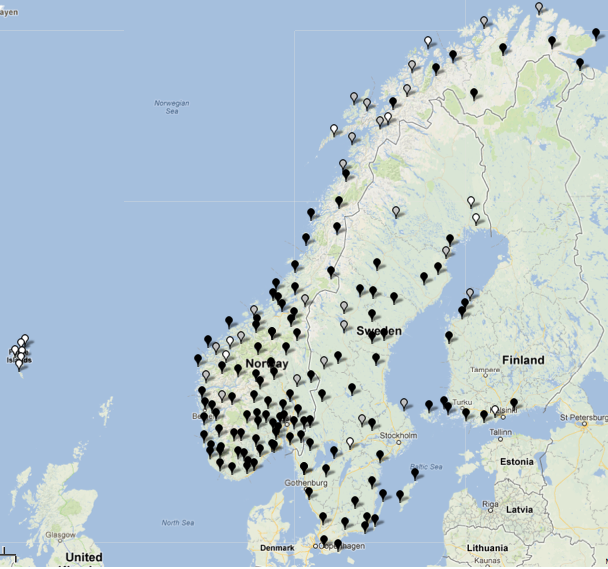
\includegraphics[width=0.9\textwidth]{../images/scanbene1}
	\caption{Scandinavian benefactive judgements (brighter dots equals higher rating)}
	\label{map:scanbene}
\end{figure}

\cite{Thrainsson.2007} shows that in Icelandic, while some verbs of creation allow free use of dative beneficiaries, other verbs of creation (including BAKE) only allow coreferential pronominal beneficiaries:

\begin{exe}
	\ex Icelandic:
	\gll {\'Eg} bakað i {mér/??þér} {köku.}\\
	I.NOM baked me.DAT/you.DAT cake.ACC.\\
	\trans `I baked myself/you a cake \citep[4.155]{Thrainsson.2007}.'
\end{exe}


Among West Germanic languages (English, Dutch, and German), English and German both have productive benefactives. In Dutch, the benefactives are restricted to a small class of fixed expressions mostly involving food: 
``In standard Dutch, this so-called benefactive use of the DOC is a near obsolete phenomenon. Apart from a handful of exceptions, such as iemand een drankje inschenken ‘to pour someone a drink’ and iemand een maaltijd bereiden ‘to prepare someone a meal’, verbs of creation and obtaining no longer allow the double object complementation pattern in Dutch \citep{Colleman.2009}.''

\subsection{Goals and Addressees}

In Modern English, `to' phrases alternates with bare noun phrases in verbs of motion (e.g. SEND) and verbs of saying (e.g. TELL)

\begin{exe}
	\ex Verbs of Motion:
	\begin{xlist}
		\ex I sent John a package.
		\ex I sent a package to John.
	\end{xlist}
	\ex Verbs of Saying:
	\begin{xlist}
		\ex I told John a story.
		\ex I told a story to John.
	\end{xlist}
\end{exe}

There are good reasons to think that with verbs of motion, there is an ambiguity between a recipient and a goal interpretation \citep{Levinson.2005,Hovav.2008}. One of the best pieces of evidence is the availability of `where' questions with verbs of transfer (e.g. GIVE) and verbs of motion (e.g. SEND). With verbs of transfer `where' questions can only have a locative interpretion (i.e. the location where the transfer takes place). With verbs of motion, a goal interpretation is also available, suggesting that `to' can be ambiguous between a goal and recipient interpretation, but only with certain types of verbs.

\begin{exe}
	\ex A: Where did you send the book?
	\begin{xlist}
		\ex[ ]{B: To my sister.}
		\ex[ ]{B: At the post office.}
	\end{xlist}
	\ex A: Where did you give the book?
	\begin{xlist}
		\ex[*]{B: To my sister.}
		\ex[ ]{B: At the post office.}
	\end{xlist}
\end{exe}

Another piece of evidence comes from cross-linguistic comparison. As mentioned above, languages with synthetic dative case mostly do not allow recipients to be introduced with prepositional phrases. However, verbs of motion can introduce goal arguments with prepositional phrases. These arguments pattern like prepositional objects, in so far as the theme (usually) precedes the goal prepositional phrase. The same property holds of addressees, although the order of prepositional phrase and clausal objects is reversed (i.e. prepositional phrase -- speech clause). Indeed, in Swedish verbs of saying only allow for prepositional objects \citep{Lundquist.2013b}. In Old English, there are no examples of verbs of transfer occuring with `to' or West Germanic `on' \citep{McFadden.2002}. However, both verbs of motion and verbs of saying do co-occur with directional prepositions from an early point, suggesting that addressees as well as goals provide a more muddled picture of ditransitives.

\begin{exe}
	\ex Old English, Verb of Motion:
		\gll And he asende hi to Bethlem.\\
		and he.NOM {sent out} them.ACC to Bethlehem.\\
		\trans `And he sent them out to Bethlehem \citep[cowsgosp:2.8.77]{Taylor.2003}.'
	\ex Old English, Verb of Saying:
		\gll \& cwaeð to him \ldots\\
		and said to him \ldots\\
		\trans `and said to him \ldots \citep[cowsgosp:4.6.169]{Taylor.2003}.'
\end{exe}

The main conclusion of this section is that recipient ditransitives form the core case of non-prepositional object ditransitive constructions. Other constructions involving non-recipient theta roles (e.g. benefactives), other case marking patterns, or ambiguity in theta role (e.g. verbs of motion and saying) provide a marginal or muddled picture of ditransitive structures. Therefore, this dissertation focuses on the nature of the core ditransitive phenomenon, namely recipient ditransitives. The next chapter will argue that all of the Germanic languages share a similar syntax for recipient ditransitives that is distinct from prepositional object constructions.
\chapter{A Morphological Analysis of Dative Shift}
Since at least \cite{Kayne.1975}, a formal relationship between prepositions and case markers has been identified. Kayne's work focused on the relationship between prepositions and case marked clitics in French, where he noticed that full noun phrase recipients introduced by prepositions alternated with dative case marked clitics. Kayne suggested that the ``prepositions'' in these cases be analysed as analytic case markers, so that both the full noun phrases and the prepositions shared teh property of having dative case.

INSERT EXAMPLES HERE

The dative clitics are restricted to recipient contexts, with goals being introduced by locative clitics.

INSERT EXAMPLES HERE

There was additional evidence that these analytic dative phrases did not behave like prepositional phrases in so far as their behaviour in fronting, secondary predication (LOOK UP FACTS)

INSERT EXAMPLES HERE

Further work on the behaviour of various ``prepositional phrases'' in French (CITATIONS) showed that there was no clear dividing line between ``prepositional'' and ``analytic case markers''. Instead, it seemed that there were a set a properties associated with ``prepositional phrases'' and another set of properties associated with ``case markers'', but that various constructions showed different mixtures of these properties (some more prepositional and some more like case markers).

INSERT TABLE FROM CITATIONS

\cite{Asbury.2007} provides an analysis that solves this problem, namely removing the syntactic distinction between case and prepositions (at least for non-structural cases, i.e. for all cases other than nominative and accusative). Under this analysis, dative case and prepositions are the same syntactic objects, which she calls a KP (following CITATION). The K head of a KP are the same syntactic object in both adpositional phrases and case marked phrases, but can have different morphological realisations. Differences between case and prepositional phrases would then reduce to either morphological differences (e.g. how phonological attached the K head is to other elements in its complement) or to the base generated position of the KP (e.g. adjunct vs argument position). Since prepositions and case markers are not intrinsically distinct objects in this system, it is to be expected that various constructions would partake of a mixture of prototypical prepositional and prototypical case marking properties.

In Germanic, English, Dutch, Afrikaans, Frisian, Norwegian, Swedish, Danish and Faroese all show a pattern that I will call dative shift (following CITATION). This pattern can be identified by the occurance of recipients both as a bare noun phrase and being introduced by a prepositional element (`to', 'aan' or `til').  

INSERT EXAMPLES HERE

Most of the previous literature (CITATIONS) has assumed that these elements are prepositional object constructions (of the form discussed above). ADD IN REFERENCE TO TAKANO. In this chapter, I argue that instead the same analysis that Kayne suggested for French should be adopted, namely that `to', `aan' and `til' should be analysed as realisations of a dative K head. Given that I just suggested that there was no syntactic difference between prepositions and case markers, it would be reasonable to ask what the practical import of this claim is. By arguing that these are actually dative KPs, I suggest that, just like dative recipients in languages without dative shift (e.g. German, Icelandic and Yiddish), the languages with dative shift base generate their recipients above the theme and derive theme--recipient word orders via scrambling. A consequence of this analysis is that the theme--`to' marked recipient orders in dative shift languages are \textbf{not} examples of prepositional object constructions. However, the syntax of recipient phrases recieves a parsimonious analysis in so far as the syntax of active recipient ditransitives is identical across the Germanic languages (although there are differences in dative case morphology).

DISCUSS FULL ANALYSIS FOR MODERN ENGLISH HERE (I.E. CONTEXTUAL ALLOMORPHY/CLITICISATION, ETC.)

In the next section, I provide relevent evidence from the non-English languages for the analysis presented above. The rest of this chapter will focus on mostly on English (since that is the language that has recieved the most attention in looking at dative shift) and argue in the following way. First, a transformational account of English dative shift with recipients is licensed (namely the objections that have been brought since at least \citet{Oehrle.1976} are answerable). Then, I showthat the current analysis is consistant with the acceptability judgements given for a number of constructions in modern English (namely asymmetric c-command tests and interactions with purpose clauses). Finally, I present evidence from Middle English that demonstrates that only the analysis given above is capable of accounting for the pattern of data found in Middle English. Given that the analysis is essential for Middle English and is compatible with the Modern English data, I conclude, following Occam's Razor, that the same analysis applies throughout.


\chapter{The Transformational Nature of English Dative Shift}
\section{Cross-linguistic Evidence}
While the dative shift in languages other than English has recieved less attention, there has still been a substatial amount of work on the topic. To the extent that there has been direct comparison, the other languages seem to mostly share the same properties as English (e.g. the asymmetric c-command facts seem to be the same CITATIONS). However, there are some differences between Modern English and these languages that are worth discussing.

First, there are a number of Scandinavian languages/dialects in which dative shift is present, but dative case has not been completely lost. In these languages, overtly marked dative case phrases alternate with prepositional phases marked with `til' (CITATION). As argued above for French, the back and forth between dative case phrases and prepositional phrases is suggestive of an abstract unification of the two topics.

INSERT EXAMPLES HERE

Secondly, Afrikaans shows an interesting behaviour in passivisation. It has been known since \cite{Zaenen.1985} that dative marked noun phrases can rise to subject position in languages like Icelandic (see REFERENCE for further discussion of this phenomenon). In Afrikaans, a recipient marked with `aan' can occur in the subject position of a passive, patterning like a dative case marked element and not like a prepositional object.

INSERT EXAMPLES HERE

Finally, the distribution of the ``prepositional'' recipient in Dutch is problematic for a prepositional object analysis. In Dutch, the ``prepositional'' recipient can occur in both the recipient--theme and theme--recipient order. The bare recipient is restricted to the recipient--theme order. That there is not a one--to--one relationship between word order and marking is problematic for the prepositional object analysis in so far as that analysis is predicated on the ``prepositional'' recipient construction being associated with the theme--recipient word order. This situation is strikingly similar to the situation in Middle English and a further discussion of this phenomenon will occur at the end of this chapter.

INSERT EXAMPLES HERE

\section{Countering Arguments Against Transformation}

Many of the objections to a transformational account rely on the confusion brought about by combining recipient and non-recipient ditransitives in the same analysis. As discussed in the previous chapter, there is good cross-linguistic evidence that non-recipient ditranstives have a different structure than recipient ditransitives (and are therefore not probative of recipient transformations). As discussed above \cite{Levinson.2005} and \cite{Hovav.2008} show that there are (at least) two `to's in English: one that introduces recipients and one that introduces goals. Any argument that uses verbs of motion (e.g. SEND) is going to run afoul of this ambiguity.

Another argument against a transformational account has relied on the existance of verbs which do not allow for `to' marking (e.g. COST, see \citet{Levin.1993} for a list).

INSERT EXAMPLES HERE

Many of these verbs in languages like German and Icelandic also lack dative recipients (i.e. they are double accusative verbs). 

INSERT EXAMPLES HERE

Some of these verbs are simply small clauses (e.g. verbs of naming), where dative case would be unexpected. The other main class are verbs of billing. The double accusative forms in German suggest that these are probably not standardly ditransitive, but instead involve a direct object recipient/source and then an adjuct measure term. The fact that the second argument can be questioned with ``how much'' is suggestive of a measure interpretation.

INSERT EXAMPLES HERE

A third argument against transformational accounts relies on purported differences in interpretation between the two word orders. One of the interpretive differences is the existence of a completion implicature in the recipient--theme order.

INSERT EXAMPLES HERE

\cite{Hovav.2008} show that this completion implicature is actually the product of verbal aspect and not directly attributable to the order of the objects.

INSERT THEIR EVIDENCE HERE

\cite{Oehrle.1976} demonstrated that there were a number of different type of recipient interpretations associated even with verbs like GIVE. He argued that one of the interpretations was only available in the recipient--theme order. This intrepretation involves abstract possession. The classic example is given below:

\begin{exe}
	\ex Nixon gave Mahler a book.
	\begin{xlist}
		\ex[ ]{Nixon gave Mahler a physical object (namely a book)}
		\ex[ ]{Nixon gave Mahler an idea (that Mahler wrote into a book)}
	\end{xlist}
	\ex Nixon gave a book to Mahler.
	\begin{xlist}
		\ex[ ]{Nixon gave Mahler a physical object (namely a book)}
		\ex[*]{Nixon gave Mahler an idea (that Mahler wrote into a book)}
	\end{xlist}
\end{exe}

These abstract interpretations inevitably involve coercing the verb into a verb of creation, since the abstract entity always comes into being by the act of giving. \cite{Frey.2001} shows that in German indefinite objects under verbs of creation have to remain in base position (i.e. they must occur to the right of manner adverbs).

INSERT EXAMPLES HERE

This means that at LF these objects need to be in their base position. Thus, they are obligatorily interpreted as scoping under the recipient \citep{Bruening.2010b}.

INSERT EXAMPLES HERE

The same interpretive pressure exists in cases of idioms. Under the assumption that at LF idiomatic objects need to form a constituent with the verb in order to receive an idiomatic interpretation, scrambled idiomatic objects would need to obligatorily reconstruct promoting the recipient--theme order. Under the assumption that reconstruction is costly, there must be some countervailing pressure that would motivate the scrambling (see \citep{Bruening.2010,Bruening.2010b,Bruening.2014} for a discussion of these issues).

INSERT EXAMPLES HERE

If we assume that scrambling needs to be motivated, it is worthwhile to see what sorts of properties motivate scrambling. As just discussed, semantic requirements can be involved (i.e. locational restrictions on interpretation). \cite{Bresnan.2007} show that prosodic and discourse factors also play a large role in deciding whether or not to scramble. Some of these properties were seen above in German, which had a very strong influence of discourse givenness/prosodic stress on the availability of scrambling. Bresnan et al. found a similar tendency in English, where given material was more likely to occur to the left of new material, although the results were less categorical than has been described for German. One way of accounting for this is to claim that there are a set of (universal) harmonic patterns concerning discourse, prosodic and semantic factors that speakers try to optimise over. \cite{Bresnan.2010} suggest the following set of harmonic preferences:

INSERT HARMONIES

These preferences can be in competition (e.g. if there is a long animate phrase and a short inanimate phrase). Different languages seem to have different baselines (i.e. how likely the theme--recipient and recipient--theme orders all else being equal) as well as different weighting for the various harmonic scales (e.g. one language could heavily weight prosodic concerns, while another heavily weights givenness). The availability of different weightings can explain why English does not show the same categorical prohibition of theme--recipient orders with new information stress that was seen in German. While both German and English disprefer scrambling new themes, the weight of the dispreference is different in the two languages, such that in German the dispreference is enough for speakers to judge such sentences ungrammatical, while in English they are merely disprefered.

\cite{Bresnan.2010} and earlier work identify that these preferences can vary by verb and that these preferences (and their concomitant frequencies in corpora) closely track speakers gradient acceptability judgements. This variation provides a counter argument against one of the final oppositions to a transformational account (namely the existence of verbs that only occur in the theme--recipient order, e.g. DONATE). \cite{Levin.2010} suggests that these verbs are simply cases where the baseline preference for the theme--recipient order is so high that no other properties are able to reduce the preference enough to license the recipient--theme order. It has been note that these verbs tend to be verbs that were borrowed from Romance languages, which have exactly this property (namely that the theme--recipient order is overwhelmingly dominant). In the Romance languages, however, there is evidence that even though the theme--recipient order is dominant, it is still derived, since the same scrambling constraint discussed for German holds (at least in Italian). In Italian, even though theme--recipient orders are dominant, in the answer to theme wh-questions, the recipient--theme order is obligatory.

INSERT EXAMPLES HERE

Thus, the grammar is able to generate recipient--theme orders with verbs like DONATE, but such forms are judged unacceptable, because of the verb (class) specific baseline propensities associated with the verbs. This explains why there is a great deal of interspeaker variation in which verbs show this property \citep{Levin.1993}, since it involves learning lexically specific information about construction probabilities. CITATION suggested that if enough other properties promote the recipient--theme order (e.g. animate pronominal recipients with heavy theme) then the recipient--theme order becomes better.

\begin{exe}
	\ex 
	\begin{xlist}
		\ex[*]{John donated the museum a painting.}
		\ex[?]{John donated her his left kidney.}
	\end{xlist}
\end{exe}

Finally, these harmonic pressures can also provide some insight into Person Case Constraint effects in English \citep{Haspelmath.2004}. The PCC seems to only hold in the recipient--theme order in English, although the judgements are quite variable.

\begin{exe}
\ex \cite[ex 29]{Haspelmath.2004}
\begin{xlist}
\ex[ ]{They showed me it.}
\ex[?]{They showed her it.}
\ex[??]{They showed her him.}
\ex[*]{They showed her me.}
\end{xlist}
\ex 
\begin{xlist}
\ex[?]{They showed it to me.}
\ex[ ]{They showed it to her.}
\ex[ ]{They showed him to her.}
\ex[ ]{They showed me to her.}
\end{xlist}
\end{exe}

Many dialects of English (including most historical dialects) essentially require unstressed theme pronouns to precede any kind of recipient as seen in corpus results (e.g. \cite{Bresnan.2007} or historical work discussed below). The main cause for the unavailability of the theme pronoun in the recipient--theme order is the strong preference for scrambling theme pronouns, which is also seen in German, where theme pronouns obligatorily precede recipients. 

INSERT EXAMPLES HERE

For PCC effects in English, we again have an interaction between two harmonic pressures, namely having theme pronouns first versus having salient animate entities first. The exception to theme pronoun first rule are cases where the recipient is more salient than the theme (i.e. 1st/2nd recipient; 3rd theme). In these cases, the preference for having salient entities before non-salient entities seems to override the preference for theme pronouns to scramble.
\section{Discursus on Nominalisation}
Another piece of evidence that has been brought against a transformational account is the behaviour of recipients in nominalisations. In English, true nominalisations (as opposed to verbal gerunds) do not allow bare objects.

\begin{exe}
	\ex 
	\begin{xlist}
		\ex[ ]{The eating of pizza}
		\ex[*]{The eating pizza}
	\end{xlist}
\end{exe}

It has been noticed that recipients cannot occur in nominalisations with `of', but must be marked with `to'.

\begin{exe}
	\ex
	\begin{xlist}
		\ex[ ]{The giving to children of candy/The giving of candy to children}
		\ex[*]{The giving of children (of candy)/The giving (of candy) of children}
	\end{xlist}
\end{exe}

This behaviour is entirely to be expected under the analysis presented here. Since recipients never receive accusative case and accusative case is the only case that is replaced by genitive in nominalisations, it is expected that recipients, which are marked with dative case, cannot be introduced by genitive `of'. However, if we look at other Germanic languages (especially languages that have synthetic dative case), dative noun phrases are prohibited from occurring within nominalisations at all (CITATION).

INSERT EXAMPLES HERE

This prohibition against datives within nominalisations is not universal. For example, Russian allows dative arguments within nominalisations (CITATION).

INSERT EXAMPLES HERE

The same availability of prepositional dative recipients in nominalisations is found in other Germanic languages with dative shift.

INSERT EXAMPLES HERE

Given that learners need to determine how large the scope of nominalisation is, since Russian allows dative phrases and German does not, it is crucial to think of what evidence the learner has available. In languages without dative shift, there is no surface similarity between recipients and goals, so goals provide no evidence for the behaviour of recipients. However, once dative shift has been acquired there are some forms which are surface ambiguous between a recipient and goal interpretaion (e.g. ``The sending of packages to Mary''). I propose that languages with dative shift acquire the ability to license recipients in nominalisations from misinterpreting older speakers production of goals in nominalisations as nominalisations with recipients, thus giving evidence for the availability of recipients in nominalisations in general.
\chapter{Modern American Evidence for Scrambling}
Binding asymmetries provide some of the clearest evidence for the internal structure of English ditransitive clauses. \cite{Barss.1986} showed that in the recipient--theme order the recipient systematically asymmetrically c-commands the theme. \cite{Aoun.1989} showed that in the theme--recipient order the theme systematically asymmetrically c-commands the recipient.  Anaphor Binding, Superiority and Negative Polarity all show the surface c-command possibilities, in which the leftmost element asymmetrically c-commands the rightmost element (examples adapted from \cite{Aoun.1989}).
\newpage
\begin{exe}
\ex Anaphor Binding
\begin{xlist}
\ex Recipient--theme: I showed Mary herself (in the mirror).
\ex Recipient--theme: *I showed herself Mary (in the mirror).
\ex Theme--recipient: I showed Mary to herself (in the mirror).
\ex Theme--recipient: *I showed herself to Mary (in the mirror).
\end{xlist}
\ex Superiority
\begin{xlist}
\ex Recipient--theme: Who did you give which check?
\ex Recipient--theme: *Which paycheck did you give who?
\ex Theme--recipient: Which check did you give to who?
\ex Theme--recipient: *Who did you give which check to?
\end{xlist}
\ex Negative Polarity
\begin{xlist}
\ex Recipient--theme: I showed no one anything.
\ex Recipient--theme: *I showed anyone nothing.
\ex Theme--recipient: I showed nothing to any one.
\ex Theme--recipient: *I showed anything to no one.
\end{xlist}
\end{exe}

However, when looking at binding tests that allow for reconstruction (quantifier binding and each...the other), the recipient binding the theme is (marginally) possible in the theme--recipient order. In the recipient--theme order, the binding relationship is completely fixed. 

\begin{exe}
\ex Quantifier Binding
\begin{xlist}
\ex Recipient--theme: I gave every worker$_i$'s mother his$_i$ paycheck.
\ex Recipient--theme: * I gave his$_i$ mother every worker$_i$'s paycheck.
\ex Theme--recipient: I gave every worker$_i$'s paycheck to his$_i$ mother.
\ex Theme--recipient: ? I gave his paycheck to every worker$_i$'s mother.
\end{xlist}

\ex Each...the other
\begin{xlist}
\ex Recipient--theme: I showed each man the other's friend.
\ex Recipient--theme: * I showed the other's friend each man.
\ex Theme--recipient: I showed each man to the other's friend.
\ex Theme--recipient: ? I showed the other's friend to each man.
\end{xlist}
\end{exe}

As discussed above concerning recipient ditransitives in Japanese, \cite{Takano.1998} showed that the Japanese binding facts are identical to the English facts. When the dative recipient precedes the accusative theme, the recipient can bind the theme, but the theme cannot bind the recipient.
\begin{exe}\ex \cite[ex 7]{Takano.1998}
\begin{xlist}
\ex[ ]{\gll Mary-ga [subete-no gakusei]$_{i}$-ni [soitu$_{i}$-no sensei]-o syookaisita\\
Mary-NOM all-GEN student-DAT he-GEN teacher-ACC introduced\\
\trans `Mary introduced every student to his teacher.'}
\ex[*]{\gll Mary-ga [soitu$_{i}$-no sensei]$_{i}$-ni [subete-no gakusei]-o syookaisita\\
Mary-NOM he-GEN teacher-DAT all-GEN student-ACC introduced\\
\trans `Mary introduced his teacher to every student.'} 
\end{xlist}
\end{exe}%8 - Japanese scope theme--recipient
When the accusative theme precedes the dative recipient, however, both binding relationships are possible, with the recipient's binding of the theme degraded, but grammatical. This marginal response parallels the marginal acceptability of the recipient's binding of the theme in English theme--recipient clauses.
\begin{exe}\ex \cite[ex 7]{Takano.1998}
\begin{xlist}
\ex[ ]{\gll Mary-ga [subete-no gakusei]$_{i}$-o [soitu$_{i}$-no sensei]-ni syookaisita\\
Mary-NOM all-GEN student-ACC he-GEN teacher-DAT introduced\\
\trans `Mary introduced every student to his teacher.'}
\ex[?]{\gll Mary-ga [soitu$_{i}$-no sensei]$_{i}$-o [subete-no gakusei]-ni syookaisita\\
Mary-NOM he-GEN teacher-ACC all-GEN student-DAT introduced\\
\trans `Mary introduced his teacher to every student.'} 
\end{xlist}
\end{exe}

Scope freezing \citep{Aoun.1989,Bruening.2001,Bresnan.2007} is another asymmetry between the recipient--theme and theme--recipient word orders. In the recipient--theme order, the theme is apparently unable to QR over the recipient in order to bind into it. 

\begin{exe}
\ex \cite[ex 2]{Bruening.2001}
\begin{xlist}
\ex I gave a child each doll. \hfill \textit{a} \textgreater \  \textit{each}, *\textit{each} \textgreater \ \textit{a}
\ex I gave each doll to a child. \hfill \textit{a} \textgreater \  \textit{each}, \textit{each} \textgreater \ \textit{a}
\end{xlist}
\end{exe}
The same unavailability of QR has been noticed in general for German \citep{Frey.1993}. 
\begin{exe}
\ex \cite[exx 22 \& 21]{Frey.1993}
\begin{xlist}
	\ex \gll DASS er mindestens einem Gast fast jedes Geschenk \"{u}berreichte\\
	that he.NOM {at least} one.DAT guest almost every.ACC gift hand.PAST\\
	\trans `that he handed at least one guest almost every gift (\textit{one} \textgreater \ \textit{every}, *\textit{every} \textgreater \ \textit{one})'
	\ex \gll DASS er mindestens ein Geschenk fast jedem Gast \"{u}berreichte\\
	that he.NOM {at least} one.ACC gift almost every.DAT guest hand.PAST\\
	\trans `that he handed at least one gift to almost every guest (\textit{one} \textgreater \ \textit{every}, \textit{every} \textgreater \ \textit{one})'
\end{xlist}
\end{exe}

Concerning German, \cite[44]{Beck.1996} proposes "that because scope order can be made clear at S-Structure [via scrambling], it has to be, so S-Structural c-command mostly reflects semantic scope." This proposal can be captured by treating A-scrambling as an overt version of QR \citep{Tonoike.1997,Abe.2005,Miyagawa.2006}.

\cite{Hallman.2015} provides additional evidence supporting a transformational account of ditransitives relying the ability of recipient to control into purpose clauses, I report here the purpose clause facts that motivated his analysis. Hallman showed that in both the recipient--theme and theme--recipient orders, the recipient is able to bind PRO in the purpose clause and the theme is able to bind the empty category object. Crucially, this means that the recipient needs to be higher than $\bar{V}$, which is the site of purpose clause attachment.
\begin{exe}
\ex \cite[exx 6 \& 7]{Hallman.2015}
\begin{xlist}
\ex Mary gave John$_{i}$ a puppy$_{k}$ [PRO$_{i}$ to play with e$_{k}$].
\ex Mary gave a puppy$_{k}$ to John$_{i}$ [PRO$_{i}$ to play with e$_{k}$].
\end{xlist}
\end{exe}%12 - Recipient--theme and theme--recipient purpose clauses

This is crucially different from the behaviour of prepositional objects in prepositional object constructions (e.g. as introduced by PUT). The prepositional objects scope under the purpose clause and cannot control into it.

INSERT EXAMPLES HERE

In (\ref{ex:comparison-trees}), I show trees of both the scrambling analysis (following \cite{McGinnis.1998} scrambling structure) pursued here and Hallman's analysis (involving an internal passivisation option, see \citet{Larson.1988}). In both cases, the recipient scopes over the purpose clause (unlike with locative phrases, where the locative PP scopes under the purpose clause). However, Hallman points out that his analysis requires further operations to correctly predict the word order of the clause (\textit{to}-marked recipient and then purpose clause), since the purpose clause is right attached inside of the right attached recipient phrase adjunct (which is right attached in parallel with ``by'' phrases in main clause passives). Under the scrambling analysis, the word order falls out without any alterations, since the recipient is still in the left attached specifier of the applicative phrase.

\begin{exe}
\ex \label{ex:comparison-trees}
\begin{xlist}
\ex Scrambling Analysis \\
\xymatrix@=2pt{
 & vP\ar@{-}[dl]\ar@{-}[dr]\\
DP\ar@{-}[d] & & \bar{v}\ar@{-}[dl]\ar@{-}[dr]\\
\text{Mary} & \text{v} & & ApplP\ar@{-}[dl]\ar@{-}[dr]\\
 & & DP\ar@{-}[d] & & \bar{Appl}\ar@{-}[dl]\ar@{-}[dr]\\
 & & \text{the book$_{i}$}\ar@{<-}@(dl,dl)[ddrrr] & DP\ar@{-}[d] & & \bar{Appl}\ar@{-}[dl]\ar@{-}[dr]\\
 & & & \text{to John} & Appl & & VP\ar@{-}[dl]\ar@{-}[dr]\\
 & & & & & DP_{i} & & \bar{V}\ar@{-}[dl]\ar@{-}[dr]\\
 & & & & & & V\ar@{-}[d] & & CP\\
 & & & & & & \text{give}& & \text{Op$_{k}$ PRO$_{i}$ to play with t$_{k}$}}
\ex Hallman's Analysis \\
 \xymatrix@=2pt{&vP_{1}\ar@{-}[dl]\ar@{-}[dr]\\
DP\ar@{-}[d] && \bar{v_{1}}\ar@{-}[dl]\ar@{-}[dr]\\
\text{Mary}&v_{1}\ar@{-}[d]&&vP_{2}\ar@{-}[dl]\ar@{-}[dr]\\
&CAUSE&\Delta&&\bar{v_{2}}\ar@{-}[dl]\ar@{-}[dr]\\
&&&\bar{v_{2}}\ar@{-}[dl]\ar@{-}[dr]&&PP\ar@{-}[d]\\
&&v_{2}&&VP\ar@{-}[dl]\ar@{-}[dr]&\text{to John}\\
&&&DP\ar@{-}[d]&&\bar{V}\ar@{-}[dl]\ar@{-}[dr]\\
&&&\text{a picture}&V\ar@{-}[d]&&CP\ar@{-}[d]\\
&&&&\text{HAVE}&&\text{Op$_{k}$ PRO$_{i}$ to play with t$_{k}$}\\}
\\
\end{xlist}
\end{exe}%13 - Tree with V' attached purpose clause

This section provided some evidence from Modern English that is suggestive that the scrambling account is correct. However, they rely on complex judgements involving differences in gradient judgement in matters of scope and control. In the next section, I provide quantitative evidence from historical data that demonstrates that the scrambling account is necessary to account for Middle English data. Since there is suggestive evidence supporting scrambling in Modern English, and conclusive evidence in Middle English, the most parsimonious assumption is that the scrambling analysis is still operative in Modern English as well.
\chapter{Historical Evidence for the Scrambling Account}
As discussed above, Old English had both recipient--theme and theme--recipient word orders, but both word orders had recipients marked with synthetic dative case.  \cite{Polo.2002} and \cite{McFadden.2002} show that in Early Middle English, `to' with verbs like GIVE began to be used especially in dialects where the last remnants of the synthetic accusative/dative distinction had been lost (it was lost last in pronouns). The fact that recipient `to' seems to be in complementary distribution with synthetic dative case is suggestive of the fact that it came to replace the synthetic dative. \cite{Allen.1999} and \cite{McFadden.2002} both show that by 1300 at the latest all traces of the synthetic dative/accusative distinction had been lost in all attested dialects. If `to' is coming to replace the synthetic dative case marker, which is now phonologically null, it should occur in every environment that the old dative case occurred.

In order to investigate the development of `to' through the history of English, I extracted all tokens from verbs of transfer (e.g. GIVE) and verbs of future transfer (e.g. PROMISE)\footnote{INSERT LIST OF ALL VERBS} from the Penn Parsed Corpus of Middle English 2 \citep{Kroch.2000}, the Penn Parsed Corpus of Early Modern English \cite{Krochp.2004}, the Penn Parsed Corpus of Modern British English \citep{Kroch.2010}, and the York-Helsinki Parsed Corpus of Early English Correspondence \citep{Taylor.2006}. Each token was coded for order of the objects, status of each object (pronoun vs. full noun phrase), and the presence or absence of `to', as well as year of composition of the text. I will discuss the behaviour of different combinations of object status in turn, since object status had a large effect of object order.

Given the influence of pronominality on word order, the case that had the most variation in word order is when both the theme and recipient were full noun phrases (e.g. ``John gave the book (to) the boy'' or ``John gave (to) the boy the book''). As can be seen in Fig. REFERENCE, `to' increases in both the theme--recipient and recipient--theme order. Indeed, by 1400 `to' was essentially categorical in theme--recipient contexts and occurred in about 50\% of recipient--theme contexts.

INSERT FIGURE HERE

\cite{Kroch.1989} proposed the notion of the Constant Rate Hypothesis, which provided an explanation for the Constant Rate Effect. In a number of historical syntax studies (CITATIONS), comparison of a change across a number of different environments (e.g. questions and negative declaratives for do-support) found that the rate of change in each context was constant. Given the nature of the logistic model used to model the data, the constant rate means that while the probability of the variable (e.g. do-support) in each context may be different from year to year, the rate at which the probabilities change remains constant across contexts.\footnote{The logistic model converts probabilities into log-odds (i.e. the log of the odds), which has the advantage of ranging from -Infinity to +Infinitiy, unlike probabilities, which range from 0 to 1. The logistic then performs linear regression on the log-odds. The constant rate effect is that the slope of the lines in log-odds space are equal across contexts (i.e. there is no significant interaction between context and year in the model).} Kroch argued that this effect occurs because the change reflects a single change across multiple contexts. The fitted slope reflects the rate at which the single syntactic change (e.g. the loss of V-to-T raising) enters the language. The flip side of this is that seeing the constant rate effect is suggestive that only one change is occurring in multiple contexts.

Since I argue that `to' in all contexts reflects a morphological decision about the realisation of dative case (i.e. between phonologically null and `to'), I predict that the constant rate effect should be found between the theme--recipient and recipient--theme contexts. Unfortunately, another change intervenes before the change could go to completion in the recipient--theme context as can be seen in Fig. REFERENCE. The analysis given here attributes the fall in the recipient--theme context to the introduction of a new grammar that had `to' as the general realisation of dative case and a phonologically null allomorph when linearly adjacent to the verb as discussed above. Since this grammar replaces both the grammar with only a null realisation of dative case and the grammar with only `to' as the realisation of dative case, it makes evaluating for the constant rate hypothesis difficult.

In order to solve this difficulty, I assume that the rate of `to' in recipient--theme contexts reflects the probability of using the only `to' grammar times the probability of using the modern grammar. This multiplication creates a mathematical model of the rise fall pattern that can be fit statistically, and allows the contribution of the only `to' grammar (where the constant rate effect is expected) to be separated from the rise in the modern grammar (which probably has no effect outside of the recipient--theme context). As predicted, there is no significant interaction found between context (theme--recipient vs recipient--theme) and year (i.e. the data is consistent with the constant rate hypothesis).

INSERT RESULTS HERE

In order to detect the power associated with a data set of this size, I used the fitted probabilities for the slope and intercepts from the actual data and simulated a number of datasets with the same distribution of tokens over context and year, assuming various interaction sizes. I then fit the models to the simulated data in order to see how often a significant interaction was detected at different interaction sizes. The results are included in the table below.

INSERT TABLE HERE

That the data is consistent with the constant rate hypothesis is suggestive of the idea that the grammar innovated in Early Modern English had `to' as the sole realisation of dative case. If the modern grammar (or a prepositional object analysis) is assumed, the use of `to' in recipient--theme contexts is not predicted, unless they reflect cases of heavy NP shift. \cite{McFadden.2002} proposed that the rise was entirely due to an increase in the number of heavy themes and thus an increase in the rate of heavy NP shift. Another alternative analysis would be that Middle English had freer order of prepositional phrases and objects than modern English, with recipient--theme orders in Middle English derived by scrambling the prepositional object over the theme.

In order to evaluate both of these theories (heavy NP shift and prepositional object scrambling), I extracted all tokens from the corpus with an object and a prepositional phrase both following the verb (including the `to' tokens from ditransitives) and also all cases with an object and an adverb both following the verb. I then coded for the order of the object with the prepositional phrase and the adverb. INSERT DATA ON RATIO OF RECIPIENT DITRANSTIVES TO PREPOSITIONAL PHRASES. The rate of prepositional phrase/adverb preceding the noun was fairly constant and much lower than 50\% (see Fig. REFERENCE), which means that reordering of prepositional phrases in general and objects is not common (as was shown above for German).

INSERT FIGURE HERE

I also took another angle to examine if heavy NP shift could account for the high rate of `to' in recipient--theme clauses in Late Middle English. I coded objects for the number of orthographic words, which is known to be a good proxy for the prosodic weight considerations that impact heavy NP shift \citep{Bresnan.2007}. I then looked at the period from 1450 to 1700 which tracks the fall in the use of `to' in recipient--theme orders. 1450 also marks the completion of the `to' grammar in the theme--recipient order, so there was no longer any concern of the rate of the only null phonology grammar. I then tested whether or not the result could be attributed to the heaviness of the object alone, or whether there was a significant effect of year on top of phonological weight (in predicting the use of `to' in recipient--theme contexts). If the effect was entirely driven by heavy NP shift, then the results should be significantly predicted by object weight alone. However, there was actually a significant effect of year as can be seen in the Table below, suggesting that there was actually a grammatical change in the availability of `to' in recipient--theme contexts (as predicted by the analysis proposed here).

INSERT TABLE HERE

As discussed above, with theme pronouns, the theme--recipient order dominated with INSERT PERCENTAGE HERE of tokens with theme pronouns in the theme--recipient order. The use of `to' still dramatically increased in this order, although as discussed above, there was a significant number of null recipients even in the modern period (especially null recipient pronouns). These reflect the effect of cliticisation (both of the theme and the recipient) as discussed above. The effects can be seen in Fig. REFERENCE.

INSERT FIGURE HERE

I tested whether the pronominal cases behaved differently from the full noun phrases

RUN TESTS AND REPORT RESULTS HERE

\part{Passive Ditransitives}
\chapter{Locality and nominative case assignment}\label{ch:nominative-locality}
\section{Theme Passivisation with Bare Recipients}
\section{Cross-linguistic Evidence}
\chapter{Dative to nominative raising}\label{ch:dative-to-nominative}
\section{Invisible Datives}
\section{Defective Intervention}
\section{Accessible Datives}
\subsection{Normally Accessible}
\subsection{Auxiliary Controlled Accessibility}
\part{Conclusions}
\chapter{Formalisation}\label{ch:formal}
\section{Active Ditransitive Syntax}
\section{Distributed Morphology and Dative Shift}
\section{Passive Ditransitive Syntax}
\subsection{Parameterising T's Locality}
\subsection{Implementing Dative-to-Nominative Raising}
\subsubsection{Option 1: Structural Dative}
\subsubsection{Option 2: Further parameterising T}
\subsubsection{Comparison of Options}
\section{Formalising Usage Patterns}
\chapter{Historical Implications}\label{ch:history}
\section{The Rise and Fall of Dative `to'}
\section{Bare Recipients and American English}
\chapter{Conclusions and Further Implications}\label{ch:concl}
\section{Summary}
\section{Further Implications: Ergativity}
% Bibliography
\bibliographystyle{mcbride}
\bibliography{diss}

\end{document}
